% Options for packages loaded elsewhere
\PassOptionsToPackage{unicode}{hyperref}
\PassOptionsToPackage{hyphens}{url}
%
\documentclass[
]{book}
\usepackage{lmodern}
\usepackage{amssymb,amsmath}
\usepackage{ifxetex,ifluatex}
\ifnum 0\ifxetex 1\fi\ifluatex 1\fi=0 % if pdftex
  \usepackage[T1]{fontenc}
  \usepackage[utf8]{inputenc}
  \usepackage{textcomp} % provide euro and other symbols
\else % if luatex or xetex
  \usepackage{unicode-math}
  \defaultfontfeatures{Scale=MatchLowercase}
  \defaultfontfeatures[\rmfamily]{Ligatures=TeX,Scale=1}
\fi
% Use upquote if available, for straight quotes in verbatim environments
\IfFileExists{upquote.sty}{\usepackage{upquote}}{}
\IfFileExists{microtype.sty}{% use microtype if available
  \usepackage[]{microtype}
  \UseMicrotypeSet[protrusion]{basicmath} % disable protrusion for tt fonts
}{}
\makeatletter
\@ifundefined{KOMAClassName}{% if non-KOMA class
  \IfFileExists{parskip.sty}{%
    \usepackage{parskip}
  }{% else
    \setlength{\parindent}{0pt}
    \setlength{\parskip}{6pt plus 2pt minus 1pt}}
}{% if KOMA class
  \KOMAoptions{parskip=half}}
\makeatother
\usepackage{xcolor}
\IfFileExists{xurl.sty}{\usepackage{xurl}}{} % add URL line breaks if available
\IfFileExists{bookmark.sty}{\usepackage{bookmark}}{\usepackage{hyperref}}
\hypersetup{
  pdftitle={An Exam P Study Guide},
  pdfauthor={Actuary Helper},
  hidelinks,
  pdfcreator={LaTeX via pandoc}}
\urlstyle{same} % disable monospaced font for URLs
\usepackage{longtable,booktabs}
% Correct order of tables after \paragraph or \subparagraph
\usepackage{etoolbox}
\makeatletter
\patchcmd\longtable{\par}{\if@noskipsec\mbox{}\fi\par}{}{}
\makeatother
% Allow footnotes in longtable head/foot
\IfFileExists{footnotehyper.sty}{\usepackage{footnotehyper}}{\usepackage{footnote}}
\makesavenoteenv{longtable}
\usepackage{graphicx}
\makeatletter
\def\maxwidth{\ifdim\Gin@nat@width>\linewidth\linewidth\else\Gin@nat@width\fi}
\def\maxheight{\ifdim\Gin@nat@height>\textheight\textheight\else\Gin@nat@height\fi}
\makeatother
% Scale images if necessary, so that they will not overflow the page
% margins by default, and it is still possible to overwrite the defaults
% using explicit options in \includegraphics[width, height, ...]{}
\setkeys{Gin}{width=\maxwidth,height=\maxheight,keepaspectratio}
% Set default figure placement to htbp
\makeatletter
\def\fps@figure{htbp}
\makeatother
\setlength{\emergencystretch}{3em} % prevent overfull lines
\providecommand{\tightlist}{%
  \setlength{\itemsep}{0pt}\setlength{\parskip}{0pt}}
\setcounter{secnumdepth}{5}
\usepackage{booktabs}
\usepackage{amsthm}
\makeatletter
\def\thm@space@setup{%
  \thm@preskip=8pt plus 2pt minus 4pt
  \thm@postskip=\thm@preskip
}
\makeatother
\usepackage[]{natbib}
\bibliographystyle{apalike}

\title{An Exam P Study Guide}
\author{Actuary Helper}
\date{2020-01-09}

\usepackage{amsthm}
\newtheorem{theorem}{Theorem}[chapter]
\newtheorem{lemma}{Lemma}[chapter]
\newtheorem{corollary}{Corollary}[chapter]
\newtheorem{proposition}{Proposition}[chapter]
\newtheorem{conjecture}{Conjecture}[chapter]
\theoremstyle{definition}
\newtheorem{definition}{Definition}[chapter]
\theoremstyle{definition}
\newtheorem{example}{Example}[chapter]
\theoremstyle{definition}
\newtheorem{exercise}{Exercise}[chapter]
\theoremstyle{remark}
\newtheorem*{remark}{Remark}
\newtheorem*{solution}{Solution}
\let\BeginKnitrBlock\begin \let\EndKnitrBlock\end
\begin{document}
\frontmatter
\maketitle

{
\setcounter{tocdepth}{1}
\tableofcontents
}
\mainmatter
\hypertarget{an-introduction-to-set-theory}{%
\chapter{An Introduction to Set Theory}\label{an-introduction-to-set-theory}}

\hypertarget{defining-sets}{%
\section{Defining Sets}\label{defining-sets}}

Sets are collections of objects. Usually objects are placed inside curly braces and separated by commas. Here is the set with the numbers 1 and 2. We often give sets a name. This set is named ``A''. \[A=\{1,2\}\]

Objects inside the curly braces are called elements of the set. There is a special character that means ``is an element of''. Using our notation we can say that 1 is an element of A. \[1 \in A\]

We can also say that 3 is not an element of A by drawing a slash through our symbol.
\[3 \not\in A\]
We can define sets in a something called set-builder notation. Set builder notation is useful for infinite sets or sets that are hard to enumerate. Below are some examples.

We can define the even numbers as \(\{x | x \ is \  an \  even \ number\}\)

We can define hands of cards as \(\{x | x \ is \  a \ 5 \ element \ subset \ of \ a \ deck \ of \ cards\}\)

To read set builder notation we translate the ``\textbar{}'' as ``where''. So the real numbers are ``the set of x where x is a real number''.

\hypertarget{set-equality-and-subsets}{%
\section{Set Equality and Subsets}\label{set-equality-and-subsets}}

Sets are equal when they have the same elements. This means order doesn't matter in sets, \(\{1,2\} = \{2,1\}\) because they have the same elements. Also, \(\{1,1,2\} = \{1,2\}\) and we say that sets don't have duplicate elements because duplicate elements have no purpose.

A set is a subset of another set when it fits inside of it. There is a symbol that looks like \(\leq\) that means ``is a subset of''. For example \(\{1,2\} \subseteq \{1,2,3\}\). It is also true that any set is a subset of itself, so \(\{1,2\} \subseteq \{1,2\}\). In more precise terms \(A \subseteq B\) if and only if every element of A is also an element of B.

A common technique to prove that two sets are equal is to show that \(A \subseteq B\) and \(B \subseteq A\). This means there is no element in either set that does not belong to the other and the sets are equal.

\hypertarget{set-operations-and-venn-diagrams}{%
\section{Set Operations and Venn Diagrams}\label{set-operations-and-venn-diagrams}}

Just like you can add numbers together to make a new number, you can combine sets and make a new set. Let's define some sets.

\[S = \{1,2,3,4,5,6,7,8,9,10\} \\
 A = \{1,3,5,7\} \\
 B = \{2,3,4,5\}\]

\hypertarget{venn-diagram}{%
\subsection{Venn Diagram}\label{venn-diagram}}

There is a visual representation of sets called a Venn Diagram. In a Venn Diagram each set is represented by a circle. The sample space is usually represented by a large box that the circles are inside of.

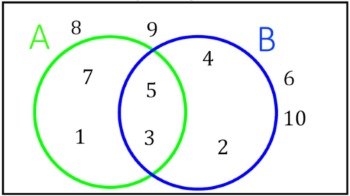
\includegraphics{Pictures/01-Sets/Venn.PNG}

\hypertarget{union}{%
\subsection{Union}\label{union}}

An element is in the union of A and B if it is in A, B, or A and B. The notation for this operation is \(A \cup B\) and it is pronounced ``A union B''. Here is the set that results from this union: \(A \cup B = \{1,2,3,4,5,7\}\)

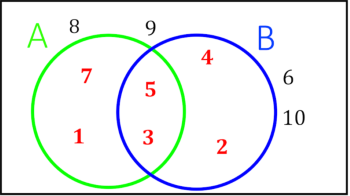
\includegraphics{Pictures/01-Sets/AUB.PNG}

\hypertarget{intersection}{%
\subsection{Intersection}\label{intersection}}

An element is in the intersection of A and B if it is in A and B. The notation for this operation is \(A \cap B\) and it is pronounced ``A intersect B''. Here is the set that results from this intersection: \(A \cap B = \{3,5\}\)

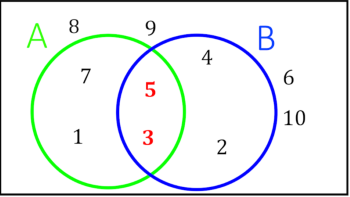
\includegraphics{Pictures/01-Sets/AcapB.PNG}

\hypertarget{complement}{%
\subsection{Complement}\label{complement}}

An element is in the complement of A if it is not in A, but is in the sample space. The notation for the complement of A is \(A^C\) and is pronounced ``A complement'' or ``the complement of A''. Here is the result of taking the complement of A: \(A^C = \{2,4,6,8,9,10\}\). Note that in general \((A^C)^C = A\).

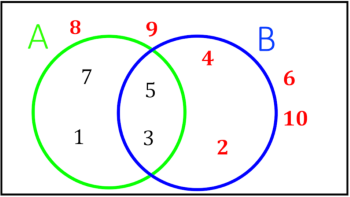
\includegraphics{Pictures/01-Sets/AC.PNG}

\hypertarget{set-difference}{%
\subsection{Set Difference}\label{set-difference}}

The set difference of A and B elements that are in A but not in B. The notation is either \(A \backslash B\) or \(A - B\) and is pronounced ``A minus B''. Here is the result of this set difference: \(A - B = \{7,1\}\). It is worth noting that \(A-B=A \cap B^C\) because the elements are in A and they are not in B.

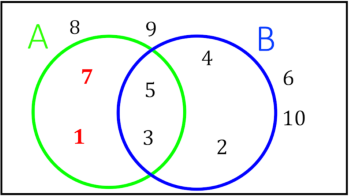
\includegraphics{Pictures/01-Sets/A-B.PNG}

\hypertarget{special-sets-and-identities}{%
\section{Special Sets and Identities}\label{special-sets-and-identities}}

\hypertarget{sample-space-and-empty-set}{%
\subsection{Sample Space and Empty Set}\label{sample-space-and-empty-set}}

The sample space is a type of special set because all other sets are subset of it. This leads to some commonsensical identities like \(A \cup S = S\) and \(A \cap S = A\). There is another special set called the empty set. This set has no elements. We could write it as \(\{\}\) but the common way to write this is \(\emptyset\). Some properties of the empty set are \(A \cup \emptyset = A\) and \(A \cap \emptyset = \emptyset\). It is also true that \(\emptyset^C = S\) and \(S^C = \emptyset\).

\hypertarget{de-morgans-laws}{%
\subsection{De Morgan's Laws}\label{de-morgans-laws}}

De Morgan's laws are formulas for the complement of a union or intersection of sets.
\[(A \cap B)^C = A^C \cup B^C \\
 (A \cup B)^C = A^C \cap B^C\]
One way of memorizing these formulas is that you bring the complement inside the parentheses to both sets and flip the union or intersection upside down.

Let's see if these laws make any sense. Let \(T\) be the set of tennis players and \(H\) be the set of hockey players. \((T \cap H)^C\) is the set of people that don't play both tennis and hockey. \(T^C \cup H^C\) is people that don't play tennis or they don't play hockey.If I don't play both sports then I either don't play tennis or I don't play hockey, so \((T \cap H)^C \subseteq T^C \cup H^C\). If I don't play tennis or I don't play hockey then it is true that I don't play both sports, so \(T^C \cup H^C \subseteq (T \cap H)^C\). This means that the sets are equal, ponder this for some time. A similar argument can be made for the complement of the union. If this is not convincing spend some time with a Venn diagram and see if you can get it to make sense.

\hypertarget{or-more-sets}{%
\subsection{3 or More Sets}\label{or-more-sets}}

\hypertarget{associativity}{%
\subsubsection{Associativity}\label{associativity}}

Just like you can add more than two numbers together you can take the intersection or union of more than two sets. For example \(\{1,2\} \cap \{2,3\} \cap \{3,4\} = \emptyset\). There are no elements in the intersection of these three sets because no number appears in all three sets, so this is the empty set. Intersections are associative, meaning \((A \cap B) \cap C= A \cap (B \cap C)\), so it doesn't matter what order you take a group of intersections in. Unions are also associative, \((A \cup B) \cup C= A \cup (B \cup C)\).

\hypertarget{distributive-property}{%
\subsubsection{Distributive Property}\label{distributive-property}}

If you mix together unions and intersections in an expression it isn't associative. Can you think of an example?
\[A \cap (B \cup C) \not= (A \cap B) \cup C\]
There are distributive formulas for situations like this.
\[A \cap (B \cup C) = (A \cap B) \cup (A \cap C) \\
 A \cup (B \cap C) = (A \cup B) \cap (A \cup C)\]
Because of this it is said that intersection distributes over unions, and that unions distribute across intersections. It is easier to remember these distributive formulas by comparing them to the way multiplication distributes over addition. \(a(b+c)=ab+ac\). Just pretend that the multiplication is an intersection and the addition is a union.

\hypertarget{messy-venn-diagrams}{%
\subsubsection{Messy Venn Diagrams}\label{messy-venn-diagrams}}

You can draw a Venn diagram for three sets with three circles. It gets a little complicated. I wouldn't bother drawing a Venn diagram for 4 sets.

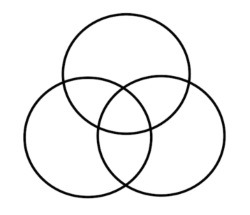
\includegraphics{Pictures/01-Sets/Venn3.PNG}
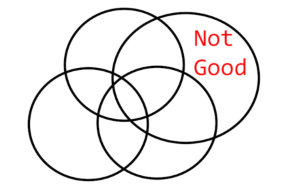
\includegraphics{Pictures/01-Sets/Venn4.PNG}

\hypertarget{counting}{%
\chapter{Counting}\label{counting}}

\hypertarget{size-of-a-set}{%
\section{Size of a set}\label{size-of-a-set}}

The set \(A = \{5,6\}\) has two elements. There is a notation to say the size of a set:
\[n(A) = 2\]
\(n\) is a function that takes in a set and outputs the number of elements in it:
\[n: Sets \to Whole \ Numbers\]
Let the sample space be \(S = \{1,2,3,4,5,6\}\). Since \(A=\{5,6\}\), \(A^C= \{1,2,3,4\}\) and \(n(A^C)=4\). There is a formula we can use for the size of the complement: \[n(A^C) = n(S) - n(A)=6-2=4\]
This is saying the size of the complement of a set is the size of the sample set minus the size of the set. I think this is pretty intuitive.

\hypertarget{principle-of-inclusion-exclusion}{%
\section{Principle of Inclusion-Exclusion}\label{principle-of-inclusion-exclusion}}

We define sets \(A\) and \(B\):
\[A = \{3,4,5\} \quad \quad B = \{4,5,6\}\]
We can see that \(A \cup B = \{3,4,5,6\}\) and \(n(A \cup B) = 4\).
Notice that \(n(A \cup B) \not = n(A) + n(B)\).

There is a special formula for the number of elements in a union called the principle of inclusion-exclusion.
\[n(A \cup B) = n(A) + n(B) - n(A \cap B)\]
We subtract \(n(A \cap B)\) from this expression because the elements of the intersection are counted twice - once in \(n(A)\), and once in \(n(B)\). Using the sets from earlier, \(A \cap B = \{4,5\}\). We can verify that the formula works by calculating \[n(A \cup B) = n(A) + n(B) - n(A \cap B) = 3 + 3 - 2 = 4\]

If the intersection of two sets is the empty set then the size of the union is the sum of the size of the sets.
\[A \cap B = \emptyset \iff n(A \cap B) = 0 \iff n(A \cup B) = n(A)+n(B)-0 = n(A)+n(B)\]
When two sets have no elements in common we call them \textbf{mutually exclusive}.

There is also a formula for the size of the union of three sets.
\[n(A \cup B \cup C) = n(A) + n(B) + n(C) - n(A \cap B)-n(B \cap C)-n(C \cap A) + n(A \cap B \cap C)\]
Consider how many times elements from each of the sections of a venn diagram with three sets are counted using the above formula. You should conclude that each element in \(A \cup B \cup C\) is counted exactly once.

\hypertarget{multiplication-principle}{%
\section{Multiplication Principle}\label{multiplication-principle}}

I have a red shirt and a blue shirt. I have a green hat, a pink hat, and a black hat. How many different shirt/hat combinations can I wear?

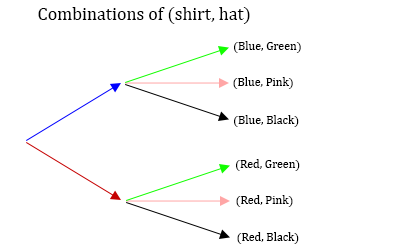
\includegraphics{Pictures/02-Counting/Tree.PNG}

The above diagram is an example of a \textbf{tree} diagram. The leaves (arrows with no arrows after them) of our tree represent the possible shirt/hat combinations. There are \(6\) possible shirt/hat combinations because there are \(2\) branches that each have \(3\) leaves which gives us \(2 \times 3 = 6\) total combinations. In general if there are \(m\) shirts and \(n\) hats there will be \(m \times n\) shirt/hat combinations because there will be \(m\) branches with \(n\) leaves. This generalizes to anything where you make two selections where the number of options in one of the selections does not depend on the other selection. For example the number of hats I can wear doesn't depend on which shirt I pick. If I decide that my pink hat is special and not to be worn with my red shirt then there are 5 combinations and the multiplication principle doesn't apply.

If I have \(4\) pairs of pants to choose from then there will be \(2 \times 3 \times 4\) shirt/hat/pant combinations. In general if you are making independent selections with \(a_1,a_2,...,a_n\) options, then the number of ways to make these selections is:
\[a_1 \times a_2 \times ... \times a_n=\displaystyle\prod_{k=1}^{n} a_k\]

\hypertarget{permutations}{%
\section{Permutations}\label{permutations}}

Permutations are all about rearranging things into ordered outcomes. For example, how many ways can we order the numbers in the set \(\{1,2,3\}\)? Let's draw a tree diagram to figure this out.

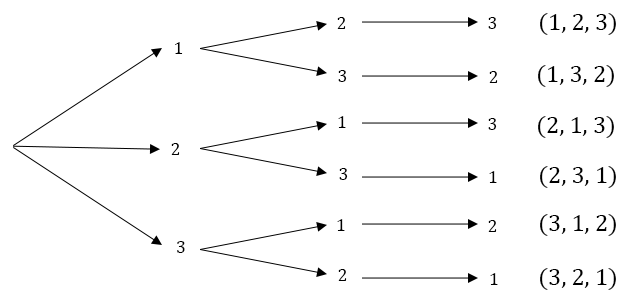
\includegraphics{Pictures/02-Counting/permute3large.PNG}

There are three options for our first selection, two options for our second selection, and one option for our third selection. The multiplication principle gives us 6 permutations of the set \(\{1,2,3\}\). Generally if \(n(A) = m\) there are \(m \times (m-1) \times ... \times 2 \times 1 = m!\) permutations of the set \(A\).

Here are some natural examples of permutations. How many possible outcomes are there in a three person race? We could imagine a set containing the different people and the outcomes of the race are the possible orders of the set. Some things not obviously involving order are permutation problems. If I bought three different chocolate bars how many ways can I give each of my three family members a chocolate bar? I think the natural way to do this is to use the multiplication principle to see that there are three options for the first chocolate bar I give away, two for the second, and one for the third. If I gave away all of the chocolates at the same time and there is no ordering it doesn't matter because I could have given the gifts away one at a time for the same set of possible outcomes.

Let's consider something more general. In a \(10\) person race how many possible outcomes are there for the top \(3\)? \(10\) people could have come in first place, there are \(9\) options for second once the first place is determined, and then \(8\) options for the third. The answer is then \(10 \times 9 \times 8=720\) using the multiplication principle. The general formula for the top \(k\) racers in an \(n\) person race is:
\[n \times (n-1) \times ... \times (n-k+1) = \frac{n!}{(n-k)!}\]
The situation for the top \(k\) racers in an \(n\) person race has it's own notation, \(P(n,k)\). \(P(n,k)\) is pronounced ``\(n\) permute \(k\)''.

\hypertarget{combinations}{%
\section{Combinations}\label{combinations}}

In permutations we consider how many possible orderings a subset of a certain size can have. What if we instead asked how many possible subsets there are of a certain size? For example, how many different ways can I pick \(2\) people from a group of \(3\) people? These problems are called combinations and the number of \(k\) element subsets of an \(n\) element set is \(C(n,k)\). An different notation that is more common is \(n \choose k\) and this is pronounced ``n choose k''. There is a relationship between permutations and combinations that we illustrate below.

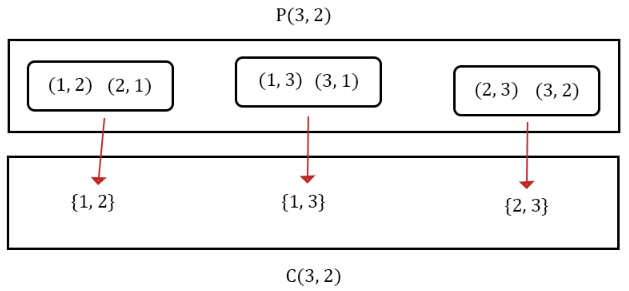
\includegraphics{Pictures/02-Counting/P(3,2)vsC(3,2).PNG}

For every set counted in \(C(3,2)\) there are two ordered pairs in \(P(3,2)\). Order doesn't matter in a combination, but it does in a permutation. If we select two people from a group of three there will be two permutations for each combination. If we select three people, there are six permutations per combination because there are six possible permutations of three people. In general we see that \(P(n,k) = C(n,k)\times k!\). Let's solve for \(C(n,k)\).

\(C(n,k) = \frac{P(n,k)}{k!} = \frac{n!}{k!(n-k)!}\)

\hypertarget{variations}{%
\section{Variations}\label{variations}}

Often a problem will involve using the multiplication principle with permutations and combinations. Consider the following:

There is a set of \(9\) distinct pigs. Three go to the market, three go to Arby's, and three go home. How many ways can this happen?

There are \(9 \choose 3\) ways to select the piggies for the market. After that selection is made there are \(6 \choose 3\) ways to select the piggies for Arby's. The remaining three piggies go home. The answer is then:
\[{9 \choose 3}\times{6 \choose 3} \times {3 \choose 3} = \frac{9!}{3!6!}\times \frac{6!}{3!3!} \times \frac{3!}{3!0!} = \frac{9!}{3!3!3!}\]
There is actually a general principle at work here. If we divide a set into mutually exclusive subsets then the number on the top is the size of the set and the numbers on the bottom are the size of the subsets.

\textbf{Is this true for dividing a set into two subsets? Why?}

A rephrasing of this question is ``How many ways can you rearrange the letters of `aaabbbccc'?'' To see that these questions are the same let each position of the letter be a piggy and assign the market, Arby's, and home to the letters a, b, and c.~Select positions in groups of three to assign the letters to.

Here is an example that combines permutations and combinations. ``How many ways could I rank my 10 favorite math problems from a list of 20 and then do 5 of them?'' There are \(P(20,10)\) possible rankings of my top 10 problems. There are \(10 \choose 5\) ways to choose from the selected problems. The answer is then:
\[P(20,10)\times{10 \choose 5} = 168,951,528,345,600\]

\hypertarget{probability-basics}{%
\chapter{Probability Basics}\label{probability-basics}}

\hypertarget{equiprob}{%
\section{Equally Likely Events}\label{equiprob}}

If we flip a coin it is said that heads and tails have the same probability because the percentage of both heads and tails tend toward \(50\%\) as the number of coin flips increases. Think of a \textbf{probability} as the percent of time an outcome occurs when many trials are performed. Here are the results of a simulation.

Number of Trials

Percent Heads

10

60\%

1,000

48.1\%

100,000

50.005\%

When we make a ``random selection'' it means that every possible selection has equal probability. For example, a randomly selected card from a deck of \(52\) cards has probability \(\frac{1}{52}\) of being a 2 of clubs.

When every possible outcome has equal probability, the formula for the probability of some subset of the outcomes is:

\[\frac{\text{Number of Selected Outcomes}}{\text{Number of Total Possible Outcomes}}\]

What is the probability of drawing 4 aces when we randomly select 5 cards from a deck? The number of ways to draw 4 aces is \({4 \choose 4} = 1\) because there are 4 aces and we must select all of them. There are 48 cards to select that are not aces which leads to \({48 \choose 1} = 48\) outcomes.

The number of ways to draw 4 aces is:
\[{4 \choose 4}{48 \choose 1} = 48\]

The number of ways to draw 5 cards is:
\[{52 \choose 5}\]

The answer is then:
\[\frac{{4 \choose 4}{48 \choose 1}}{{52 \choose 5}} = \frac{48}{2598960} = \frac{1}{54145}\]

\hypertarget{terminology}{%
\section{Terminology}\label{terminology}}

\hypertarget{sample-spaces-and-events}{%
\subsection{Sample Spaces and Events}\label{sample-spaces-and-events}}

In probability we talk about experiments, sample spaces, and events.

When we flip a coin or roll a die that is an \textbf{experiment}. Experiments have a set of possible outcomes that happen with some probability.

The set of all possible outcomes of an experiment is the \textbf{sample space}. When we flip a coin once the sample space is \(S=\{H,T\}\). When we flip a coin twice the sample space is \(S=\{HH,HT,TH,TT\}\).

\textbf{Events} represent a set of possible outcomes from an experiment. When we flip two coins there is an event for flipping two heads, \(E_\text{both heads}=\{HH\}\). There is also an event for not flipping two heads \(E_\text{not both heads}=\{HT,TH,TT\}\). An event is a subset of the sample space. It may represent a single outcome of our experiment, or it may represent several of the possible outcomes:
\[E \subseteq S\]

We can rewrite our formula for probabilities when all outcomes of an experiment are equally likely using \(n(E)\) for the number of selected outcomes.
\[\frac{\text{Number of Selected Outcomes}}{\text{Number of Total Possible Outcomes}} = \frac{n(E)}{n(S)}\]

\begin{center}\rule{0.5\linewidth}{0.5pt}\end{center}

\textbf{Example: Rolling Dice}

We roll two dice and want to calculate the probability that the dice sum to 4. Define the experiment, sample space, event, and calculate the probability of the event.

The experiment is rolling two dice.

The sample space has 36 elements, we can define it in set-builder notation:
\[\{(a,b)|a,b \in \{1,2,3,4,5,6\}\}\]
The event contains the elements of the sample space summing to 4.
\[E = \{(1,3),(3,1),(2,2)\}\]
The probability is
\[\frac{\text{Number of Selected Outcomes}}{\text{Number of Total Possible Outcomes}} = \frac{n(E)}{n(S)} = \frac{3}{36}=\frac{1}{12}\]

\begin{center}\rule{0.5\linewidth}{0.5pt}\end{center}

\hypertarget{probability-functions}{%
\section{Probability Functions}\label{probability-functions}}

There is a function called a probability function, denoted \(P\), that calculates the probability of an event. When we flip a coin twice the probability of getting a head and a tail is:
\[P(\{HT, TH\})=.5\]
For experiments where all outcomes are equally likely:
\[P(E) = \frac{n(E)}{n(S)}\]
A probability is between \(0\) and \(1\) because an event can't happen less than \(0\%\) of the time or more than \(100\%\) of the time. More formally, \(P\) is a function that takes an event as input and gives a number between \(0\) and \(1\) as output. In notation:
\[P:E \mapsto [0,1]\]

If we are being more mathematically rigorous, this rule about probabilities being between \(0\) and \(1\) is derived from some more basic assumptions and not intuition about the percentage of times something occurs. Let's talk about these basic assumptions.

\hypertarget{axiomsprob}{%
\subsection{Probability Axioms}\label{axiomsprob}}

There are three fundamental assumptions (called axioms) about probability functions from which our other laws are derived.

\textbf{First Axiom} - For an event \(E\), and probability function \(P\):
\[P(E) \geq 0\]
\textbf{Second Axiom} - For a sample space \(S\):
\[P(S)=1\]
\textbf{Third Axiom} - If \(E1, E2, ...En\) are \textbf{mutually exclusive} events:
\[P(\bigcup\limits_{i=1}^{\infty} E_{i})=P(E_1 \cup E_2 \cup...\cup En \cup...) = P(E1)+P(E2)+...+P(En)+...\]
For \textbf{two mutually exclusive} events events the third axiom is:
\[P(E_1 \cup E_2) = P(E_1)+P(E_2)\]

There are several formulas that are useful for this exam that can be derived from these axioms. We can derive the formula for the probability of the complement of an event:
\[P(A)+P(A^C) = P(A \cup A^C) = \ P(S) = 1 \ using \ Axioms \ 2 \ and \ 3\]
Since \(P(A^C)+P(A) = 1 \implies P(A^C) = 1-P(A)\).

Here are some useful formulas that can be derived from these axioms.
\[Complements: \ P(A^C) = 1 - P(A) \\
Upper \ Bound:P(A) \leq 1 \\
General \ Probability \ of \ 2 \ Unions: P(A \cup B) = P(A) + P(B) - P(A \cap B) \\
3 \ Unions: P(A \cup B \cup C) =  \\ P(A) + P(B) + P(C) - P(A \cap B)-P(B \cap C)-P(C \cap A) + P(A \cap B \cap C)\]

Notice that these formulas are the same as our formulas for the size of the set if we swap out \(P\) for \(n\) and \(1\) for \(n(S)\).

\begin{center}\rule{0.5\linewidth}{0.5pt}\end{center}

\textbf{Example: Coin Flipping and Axioms}

If we flip a coin, heads and tails are mutually exclusive events.
\[P(\{H\} \cup \{T\}) = P(\{H\})+P(\{T\}) = .5 + .5 = 1\]
We know that \(P(\{H\}), P(\{T\})=.5\) from our formula for equally likely events at the beginning of the chapter. Note that \(S = \{H\} \cup \{T\}\) so this example also illustrates that \(P(S)=1\).

\begin{center}\rule{0.5\linewidth}{0.5pt}\end{center}

\hypertarget{conditional-probability-and-independence}{%
\section{Conditional Probability and Independence}\label{conditional-probability-and-independence}}

Fluffy

Not Fluffy

Total

Cats

21

18

39

Dogs

35

26

61

Total

56

44

100

We make estimates about the overall population of pets using the results of a survey about pets. To do this we pretend that the pets in the survey represent the entire population of pets.

We can calculate the probability of a pet being fluffy using our formula for \protect\hyperlink{equiprob}{equally likely events}:
\[\frac{\text{Number of Fluffy Pets}}{\text{Total Number of Pets}} = \frac{n(\text{Fluffy})}{n(\text{Pets})} = \frac{56}{100}\]

We can calculate the probability of a pet being a fluffy cat as:
\[\frac{\text{Number of Fluffy Cats}}{\text{Total Number of Pets}} = \frac{n(\text{Fluffy} \cap \text{Cat})}{n(\text{Pets})} = \frac{21}{100}\]

We can also calculate the probability of a pet being fluffy, given that the pet is a cat:
\[\frac{\text{Number of Fluffy Cats}}{\text{Total Number of Cats}} = \frac{n(\text{Fluffy} \cap \text{Cat})}{n(\text{Cats})}=\frac{21}{39}\]
Calculating the probability of a pet being fluffy given that the pet is a cat is an example of conditional probability because in the denominator we do not include all of the possible pets, but only the cats. There is a special notation for conditional probabilities:
\[\text{Probability Pet is Fluffy given that Pet is a Cat} = P(\text{Pet is Fluffy}|\text{Pet is a Cat})\]
The general formula for conditional probabilities uses probabilities instead of set sizes. If all outcomes are equally likely either the probability or set size formula will give the same result:
\[\frac{P(\text{Fluffy} \cap \text{Cat})}{P(\text{Cat})} =  
\frac{n(\text{Fluffy and Cat})/n(\text{Pets})}{n(\text{Cat})/n(\text{Pets})} = \frac{n(\text{Fluffy}\cap\text{Cat})}{n(\text{Cat})}\]

\begin{center}\rule{0.5\linewidth}{0.5pt}\end{center}

\hypertarget{condprob}{%
\subsection{Conditional Probability Formulas}\label{condprob}}

The probability of event \(A\) given that event \(B\) has occurred is denoted \(P(A|B)\) and pronounced ``the probability of A given B''.
The general formula for this is \[P(A|B)=\frac{P(A \cap B)}{P(B)}\]

For experiments where all outcomes have equal probabilities \(P(A|B)\) can be calculated with set sizes. The derivation for forumla this was done in our example with fluffy cats. \[P(A|B)=\frac{n(A \cap B)}{n(B)}\]

We can calculate the probability of the intersection using the probability of the given event with the conditional probability. This formula is easiest to conceptualize if you imagine an event B happening with probability \(P(B)\) and then an event \(A\) happening with probability \(P(A|B)\). \[P(A|B) \times P(B) = P(A \cap B)\]

\begin{center}\rule{0.5\linewidth}{0.5pt}\end{center}

\hypertarget{independence}{%
\subsection{Independence}\label{independence}}

Events are independent if they do not influence each other. The first flip of a coin will not impact the second flip so these events are independent.

Let the event that the first card pulled without replacement from a deck is a jack be \(J_1\) and the event that the second card pulled is a jack is \(J_2\). If I pull a jack on my first try there will be less jacks in the deck for the second draw. The event \(J_1\) has an effect on \(J_2\) and these events are not independent.

\textbf{Definition of Independence}: Events \(A\) and \(B\) are said to be independent if \(P(A|B)=P(A)\).

This definition is equivalent to \(P(A \cap B) = P(A) \times P(B)\) after substitution with the \protect\hyperlink{condprob}{conditional probability formulas}. This identity has it's own name:

\textbf{Multiplication Rule for Independent Events}: If \(A\) and \(B\) are independent events then \(P(A \cap B) = P(A) \times P(B)\).

Let \(H_n\) be the event that the nth flip of a coin is heads so that \(H_2\) means the second coin flip is heads. The multiplication rule for independent events works for more than two events if all events are mutually independent so that \(P(H_1 \cap H_2 \cap H_3 \cap H_4)=P(H_1)\times P(H_2)\times P(H_3)\times P(H_4) = (\frac{1}{2})^4\).

\hypertarget{bayes-theorem}{%
\section{Bayes Theorem}\label{bayes-theorem}}

\hypertarget{bayes-theorem-intuition}{%
\subsection{Bayes Theorem Intuition}\label{bayes-theorem-intuition}}

Suppose 1\% of the population uses drugs. 98\% of drug users test positive on a drug test and 2\% of non-users test positive. What is the probability that a person testing positive for a drug test has used drugs?

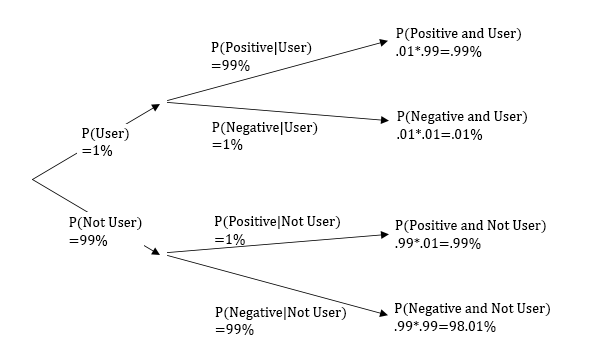
\includegraphics{Pictures/03-Probability/BayesTreeSmall.PNG}

Using the above tree diagram and the definition of conditional probability we calculate: \[P(User|Positive) = \frac{P(User \cap Positive)}{P(Positive)}= \\ 
\frac{P(User \cap Positive)}{P(Positive \cap Not \ User) + (Positive \cap User)} =\\  \frac{P(Positive|User) \times P(User)}{P(Positive|User) \times P(User)+P(Positive|Not \ User) \times P(Not \ User)} = \\
\frac{.0099}{.0099+.0099}=\frac{1}{2}\]

Let's explain these steps in more detail.

\hypertarget{law-of-total-probability}{%
\subsection{Law of Total Probability}\label{law-of-total-probability}}

In our calculation when we go from the first to the second line we use the identity \(P(Positive)=P(Positive \cap User)+P(Positive \cap Not \ User)\), but how do we know this is true?
\(Positive \cap User\) only contains drug users and \(Positive \cap Not \ User\) only contains non-users. These events are mutually exclusive so \(P(Positive \cap User)+P(Positive \cap Not \ User) = P((Positive \cap User) \cup (Positive \cap Not \ User))\) using our \protect\hyperlink{axiomsprob}{third probability axiom}. Using the distributive property for intersections with the identities
\[A^C \cup A = Sample \ Space, \quad A \cap (Sample \ Space) = A\]
we can see that:
\[(Positive \cap User) \cup (Positive \cap Not \ User) = Positive \cap (User \cup Not \ User) = \\ Positive \cap (Sample \ Space) = Positive\]
This is how we know that \(P(Positive)=P(Positive \cap User)+P(Positive \cap Not \ User)\).

There is a more general formulation of this known as the \textbf{law of total probability}:

\begin{center}\rule{0.5\linewidth}{0.5pt}\end{center}

Events \(A_1,A_2,...,A_n\) are said to be a \textbf{partition} of the sample space \(S\) if \(A_1 \cup A_2 \cup... \cup A_n=S\) and if for all \(i,j: \ A_i \cap A_j = \emptyset\). This just means that the sets \(A_1,A_2,...,A_n\) cover the whole set and there is no overlap between the sets.

If sets \(A_1,A_2,...,A_n\) partition \(S\) then for any event \(E\) we have \textbf{the law of total probability}:
\[P(E) = P(E \cap (A_1 \cup A_2 \cup ... \cup A_n)) = \\ P(E \cap A_1) + P(E \cap A_2) + ... + P(E \cap A_n) = \\ P(E|A_1) \times P(A_1) +...+ P(E|A_n) \times P(A_n)\]

Here is a visual explaining the intuition behind the equality in the first line of the equations above:

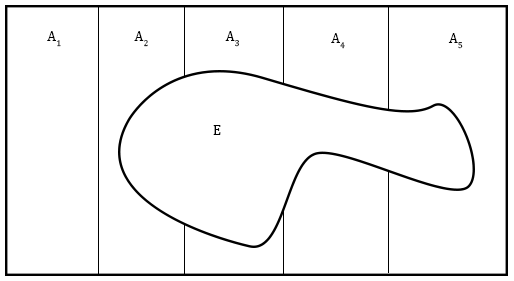
\includegraphics{Pictures/03-Probability/totalprob.PNG}

The proof of the law of total probability is outlined in our discussion of drug users.

\begin{center}\rule{0.5\linewidth}{0.5pt}\end{center}

\hypertarget{bayes-theorem-formula}{%
\subsection{Bayes Theorem Formula}\label{bayes-theorem-formula}}

\hypertarget{derivation-using-law-of-total-probability}{%
\subsubsection{Derivation Using Law of Total Probability}\label{derivation-using-law-of-total-probability}}

In our previous example every person is either a drug user or not so this partitions the sample space into two regions, \(User\) and \(Not \ User\). We can use the definition of conditional probability to say:
\[P(User|Positive)=\frac{P(User \cap Positive)}{P(Positive)}\]
We use the law of total probability in the denominator to expand it and convert all expressions of the form \(P(A \cap B)\) to expressions of the form \(P(B | A) \times P(A)\). The result is:
\[\frac{P(Positive|User) \times P(User)}{P(Positive|User) \times P(User)+P(Positive|Not \ User) \times P(Not \ User)}\]

\hypertarget{bayes-theorem-statement}{%
\subsubsection{Bayes Theorem Statement}\label{bayes-theorem-statement}}

For a partition \(A_1,A_2,...,A_n\) and event \(E\):
\[P(E|A_k) = \frac{P(E|A_k) \times P(A_k)}{P(E|A_1) \times P(A_1) +...+ P(E|A_n) \times P(A_n)}\]

\hypertarget{random-variables}{%
\chapter{Random Variables}\label{random-variables}}

\hypertarget{what-is-a-random-variable}{%
\section{What is a Random Variable}\label{what-is-a-random-variable}}

\textbf{A random variable is a number determined by chance}. What is the temperature in my city tomorrow? This is a number determined by chance, a random variable. OK sorry. I lied about a random variable being a number. Actually, \textbf{a random variable is a function} that takes an element of the sample space as input and produces a real number. What does that mean?

\begin{center}\rule{0.5\linewidth}{0.5pt}\end{center}

\BeginKnitrBlock{example}[Counting Heads]
\protect\hypertarget{exm:counthead}{}{\label{exm:counthead} \iffalse (Counting Heads) \fi{} }If you flip a coin twice the sample space is \(S=\{HH,HT,TH,TT\}\). We define a random variable \(X\) that maps the sequence of heads and tails to the number of heads. For example, \(X(HT)=1\) because there is exactly 1 head. See below that a random variable is a function that takes elements of the sample space and outputs a number.

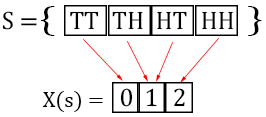
\includegraphics{Pictures/04-RV/XIsAFunction.PNG}
\EndKnitrBlock{example}

\begin{center}\rule{0.5\linewidth}{0.5pt}\end{center}

Let's return to the question of tomorrow's temperature. I said this is a random variable because it is a random number. But I thought random variables were functions, not numbers? Why did I lie to you?

\begin{center}\rule{0.5\linewidth}{0.5pt}\end{center}

\BeginKnitrBlock{example}[Tomorrow's Temperature]
\protect\hypertarget{exm:temperatures}{}{\label{exm:temperatures} \iffalse (Tomorrow's Temperature) \fi{} }The set of possible temperatures measured in degrees farenheit is the sample space \(S\). Our random variable is a function that sends a temperature in degrees farenheit to the real number that represents the temperature. Notice that there are no units for \(X(s)\), it is a real number.

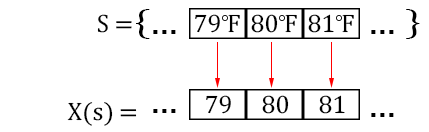
\includegraphics{Pictures/04-RV/temperatures.PNG}

See that a random variable is a function. It is just a very simple one.
\EndKnitrBlock{example}

\begin{center}\rule{0.5\linewidth}{0.5pt}\end{center}

Students can get confused about random variables because often the random variable is something simple like in the temperature example. The student then begins to overgeneralize and confuse random variables with sample spaces.

The important part of random variables isn't being able to describe them as being a function. The important part is being able to calculate the probability that tomorrow is a warm day. Let's get into that.

\hypertarget{probability-distribution-functions}{%
\section{Probability Distribution Functions}\label{probability-distribution-functions}}

\hypertarget{probability-of-an-outcome}{%
\subsection{Probability of an Outcome}\label{probability-of-an-outcome}}

We can calculate the probability of a random variable being a particular value. Let's work an example.

\begin{center}\rule{0.5\linewidth}{0.5pt}\end{center}

\BeginKnitrBlock{example}[Probability of One Head]
\protect\hypertarget{exm:unnamed-chunk-2}{}{\label{exm:unnamed-chunk-2} \iffalse (Probability of One Head) \fi{} }Again we are flipping a coin twice and \(S=\{HH,HT,TH,TT\}\). Let \(s \in S\), and \(X\) is the random variable for the number of heads. \(X(s) = 1\) when \(s \in \{HT,TH\}\). To calculate the probability of \(X(s) = 1\):
\[P(X(s)=1)=P(\{HT,TH\})=\frac{1}{2}\]
\EndKnitrBlock{example}

\begin{center}\rule{0.5\linewidth}{0.5pt}\end{center}

Even though \(X\) is a function we usually don't write it as such. Instead of saying \(X(s)=1\) we usually just write \(X=1\) and it is understood that \(X\) is a function. In our previous example we could rewrite it as \(P(X=1)=P(\{HT,TH\})=\frac{1}{2}\).

\hypertarget{probability-distribution-function-definition}{%
\subsection{Probability Distribution Function Definition}\label{probability-distribution-function-definition}}

It is common to calculate the probability of a random variable being a value \(x\), \(P(X=x)\). It is so common that we call it a ``probability distribution function'' (abbreviated \textbf{PDF}) and give it special notation.

\begin{center}\rule{0.5\linewidth}{0.5pt}\end{center}

\BeginKnitrBlock{definition}[Probability Distribution Function]
\protect\hypertarget{def:unnamed-chunk-3}{}{\label{def:unnamed-chunk-3} \iffalse (Probability Distribution Function) \fi{} }The probability distribution calculates \(P(X=x)\). There is a special way to write this, instead of using a capital \(P\) we use a lowercase \(p\) and say that:
\[p(x)=P(X = x)\]

Some properties of the probability distribution function are that the probability of an outcome is between 0 and 1, and that the sum of the probability of all possible outcomes is 1:

For \(x \in S\)

\begin{itemize}
\tightlist
\item
  \(0 \leq p(x) \leq 1\)
\item
  \(\sum p(x)=1\)
\end{itemize}
\EndKnitrBlock{definition}

\begin{center}\rule{0.5\linewidth}{0.5pt}\end{center}

The table below shows the probabilities from our coin flipping example \ref{exm:counthead}. The probabilities are between \(0\) and \(1\) and sum up to \(1\) as expected.

x

0

1

2

p(x)

.25

.5

.25

\hypertarget{cdf}{%
\section{Cumulative Distribution Functions}\label{cdf}}

Again we are flipping the coin twice and counting the heads. We can calculate the probability of \(0\) heads as \(.25\), and the probability of \(1\) head as \(.5\).

Now we can also calculate \(P(X \leq 1) = p(0)+p(1) = .25+.5=.75\). Calculations of this sort are very common, we call it the cumulative distribution function (abbreviated \textbf{CDF}). There is a special notation for this.

\begin{center}\rule{0.5\linewidth}{0.5pt}\end{center}

\BeginKnitrBlock{definition}[Cumulative Distribution Function]
\protect\hypertarget{def:unnamed-chunk-5}{}{\label{def:unnamed-chunk-5} \iffalse (Cumulative Distribution Function) \fi{} }The cumulative distribution function calculates \(P(X \leq x)\). There is a special way to write this:
\[F(x)=P(X \leq x)\]

We can calculate the cumulative distribution function by summing the probability density function:
\[F(x_0) = \displaystyle\sum_{x \leq x_0} p(x)\]
\EndKnitrBlock{definition}

\begin{center}\rule{0.5\linewidth}{0.5pt}\end{center}

We calculate the cumulative distribution function for our coin flipping example, see that the CDF is the cumulative sum of the PDF.

x

0

1

2

p(x)

.25

.5

.25

F(x)

.25

.75

1.00

In the above table we only define the CDF at points \(0,1,2\) but we can also calculate the CDF at \(.5\). \[F(.5)=P(X \leq .5) = \displaystyle\sum_{x \leq .5} p(x) = p(0) = .25\]
The CDF only changes at values where there are outcomes that happen with some probability. Understand why the graph below looks the way it does.

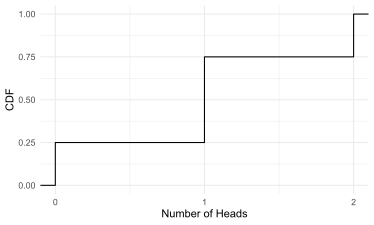
\includegraphics{Pictures/04-RV/CDFPlot.PNG}

\hypertarget{discrete-vs.-continuous-random-variables}{%
\section{Discrete vs.~Continuous Random Variables}\label{discrete-vs.-continuous-random-variables}}

So far we have only talked about flipping coins. When I flip a coin twice the only possible numbers for the heads are \(\{0,1,2\}\). This is an example of a \textbf{discrete random variable}. Discrete means that only certain numbers are possible. Plotting the possible outcomes on a number line yields a series of points.

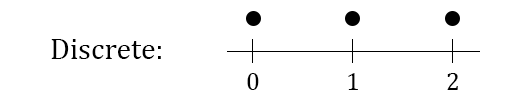
\includegraphics{Pictures/04-RV/discrete.PNG}

Some random variables are \textbf{continuous}. This means that the outcomes are intervals instead of points. The length of a cat is continuous, the length could truly be any number.

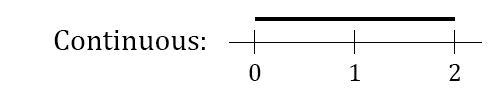
\includegraphics{Pictures/04-RV/continuous.PNG}

Some random variables are continuous and discrete \textbf{mixed} together. If my speakers volume knob must be between \(0\) and \(2\) then often my speakers will often be turned to exactly \(0\) (no sound) or \(2\) (max sound). If the volume knob is somewhere between \(0\) and \(2\) it could be turned to any number, like 1.5543\ldots, so the volume knob is a mixture of discrete and continuous.

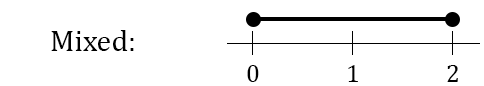
\includegraphics{Pictures/04-RV/mixed.PNG}

\hypertarget{a-bit-more-precise}{%
\subsection{A Bit More Precise}\label{a-bit-more-precise}}

In the volume knob example the possible outcomes come from the interval \([0,2]\), this sounds continuous? What about it exactly is mixed? In the CDF there is a jump at \(0\) because \(P(X \leq -.01)=0\) but \(P(X \leq 0) =\) the probability that the volume is zero.

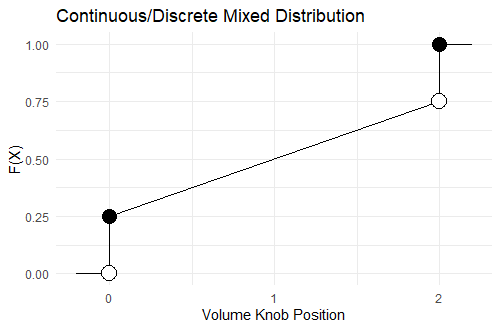
\includegraphics{Pictures/04-RV/mixedplot.PNG}

Generally discrete distributions are just going to bounce around without ever smoothly increasing over an interval. Consider the coin flipping CDF graph at the end of last section. Continuous distributions smoothly increase over intervals. Let our random variable be a randomly draw a number in \([0,1]\). The CDF smoothly increases from \(0\) to \(1\) on \([0,1]\).
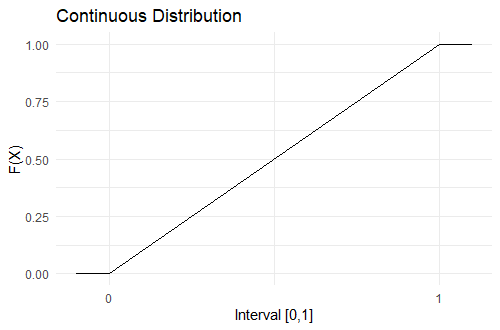
\includegraphics{Pictures/04-RV/continuousplot.PNG}

The CDF jumps at a point \(x\) when \(P(X=x)\) is nonzero, consider our volume knob example for evidence of this. A randomly selected number from \([0,1]\) is \textbf{exactly} \(.5\) with probability \(0\), so the continuous random variable has no jumps. There are infinitely many numbers in \([0,1]\) and \(.5\) is only one of these infinitely many numbers. From our formula for equally likely outcomes:
\[\frac{\text{Number of Selected Outcomes}}{\text{Number of Total Outcomes}}=\frac{1}{\infty}=0\]

We are still not telling the whole story. Continuous distributions end up using a bunch of calculus and we will discuss them in a later chapter.

\hypertarget{functions-of-discrete-random-variables}{%
\chapter{Functions of Discrete Random Variables}\label{functions-of-discrete-random-variables}}

\hypertarget{what-is-the-mean}{%
\section{What is the Mean?}\label{what-is-the-mean}}

Your friend plays a game with you where he flips a coin twice. You win \(10\$\) if both flips are heads, and lose \(4\$\) otherwise. Let's simulate some results to see if we should play this game.

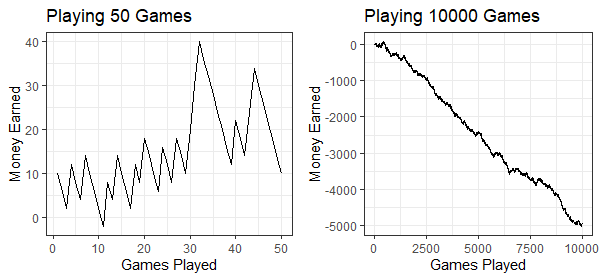
\includegraphics{Pictures/05-Expectations/Rplot02.PNG}

After \(50\) games we might think this is a fun game but in fact the odds are stacked against us. On average we lose .5 dollars per game. In our simulation notice that the average payoff approaches \(-.5\).

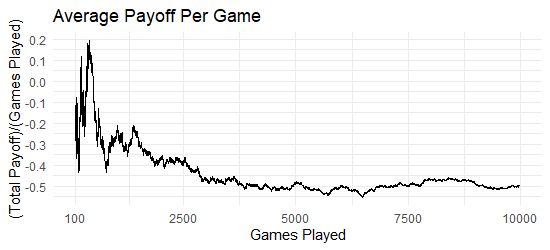
\includegraphics{Pictures/05-Expectations/averagepayoff.PNG}

We can calculate the average payoff over the \(10,000\) simulated games by adding up the payoffs and dividing by the number of games:

Games Played

Wins

Losses

10000

2501

7499

\[\frac{\sum \text{Payoff} }{\text{Number of Games}} = \frac{2501 \times 10 + 7499 \times {-4}}{10000}=-0.4986\]
We can do some rearranging:
\[\frac{2501 \times 10 + 7499 \times{-4}}{10000} = \frac{2501}{10000}(10)+\frac{7499}{10000}({-4}) = \\ \%  \text{Wins} \times 10 + \% \text{Losses} \times {-4}\]

As the number of trials increases \(\% \text{Wins}\) approaches \(P(\{HH\})\) and \(\% \text{Losses}\) approaches \(P(\{HT,TH,TT\})\). We can define a random variable \(X\) to represent the payoff with a probability distribution function of:
\[p(10) = P(\{HH\}) = .25 \\ p(-4) = P(\{HT,TH,TT\})=.75\]
We can then write the long term average payoff as:
\[{-4} \times p({-4})+10 \times p(10) = .75 \times {-4} + .25 \times 10=-.5\]
So the long term payoff of our random variable is \(.5\). When we have a random variable \(X\) that represents the payoff, we say that this is the \textbf{mean} of \(X\).

\begin{center}\rule{0.5\linewidth}{0.5pt}\end{center}

\BeginKnitrBlock{definition}[Expected Value]
\protect\hypertarget{def:expectedvalue}{}{\label{def:expectedvalue} \iffalse (Expected Value) \fi{} }The mean of a random variable \(X\) is also called the \textbf{expected value} and is denoted by \(E(X)\) or \(\mu\). To calculate the value of the mean we take the probability weighted sum of the possible values of the random variable.

\[ \mu = E(X) = \sum p(x) \times x\]
\EndKnitrBlock{definition}

\begin{center}\rule{0.5\linewidth}{0.5pt}\end{center}

Take a moment and see that the summation in our calculation is the same one performed in our calculation of the coin flipping game.

\begin{center}\rule{0.5\linewidth}{0.5pt}\end{center}

\BeginKnitrBlock{example}[Average Heads]
\protect\hypertarget{exm:unnamed-chunk-13}{}{\label{exm:unnamed-chunk-13} \iffalse (Average Heads) \fi{} }We flip a coin twice, let \(X\) be the number of heads. What is \(E(X)\)?

\[E(X) = p(0) \cdot 0 + p(1) \cdot 1 + p(2) \cdot 2 = .25 \cdot 0 + .5 \cdot 1 + .25 \cdot 2 = 1\]
\EndKnitrBlock{example}

\begin{center}\rule{0.5\linewidth}{0.5pt}\end{center}

\hypertarget{eax-b}{%
\subsection{E(aX + b)}\label{eax-b}}

Suppose we flip a coin twice. We play a game where we receive \(2\$\) for every head we flip. Let the random variable for the number of dollars we receive be \(Y\) and the random variable for the number of heads flipped be \(X\). Notice that \(Y=2X\).

Probability

.25

.5

.25

Heads

0

1

2

Dollars

0

2

4

We calculate \(E(Y)\):
\[E(Y) = .25 \cdot 0 + .5 \cdot 2 + .25 \cdot 4 = 2\]
\(E(Y) = 2\) and from example \ref{exm:counthead}, \(E(X) = 1\). This makes sense because \(Y = X-1\). What if we got \(4\) dollars or \(7\) dollars for each head? In general if we get \(a\) dollars per head:

\begin{align}
E(Y) &= .25 \cdot 0 + .5 \cdot a + .25 \cdot 2a \notag \\
&= a(.25 \cdot 0 + .5 \cdot 1 + .25 \cdot 2) \notag \\
&= aE(X) \notag
\end{align}

Let's make a new game. We still get \(2\) dollars for each head but this time we have to pay \(1\) dollar to play. Let the random variable representing the payout be \(Z\). Note that \(Z=Y-1\). We calculate \(E(Z)\):

\[E(Z) = .25 \cdot {-1} + .5 \cdot 1 + .25 \cdot 3=1\]
Notice that \(E(Z) = E(Y) - 1\) which makes sense since \(Z = Y - 1\). What if we have to pay a different amount? Let's come up with a formula for \(Z\) = \(Y-a\)

\begin{align} 
E(Z) &= .25 \cdot (0-a) + .5 \cdot (2-a) + .25 \cdot (4-a) \notag \\
&= (.25 \cdot 0 + .5 \cdot 2 + .25 \cdot 4) + a(.25+.5+.25) \notag \\
&= E(Y) - a = 2E(X)-a \notag
\end{align}

These tricks work for any random variable, not just coins. The proof of the following theorem is very similar to the calculations we have been doing.

\begin{center}\rule{0.5\linewidth}{0.5pt}\end{center}

\BeginKnitrBlock{theorem}[E(aX+b)]
\protect\hypertarget{thm:unnamed-chunk-15}{}{\label{thm:unnamed-chunk-15} \iffalse (E(aX+b)) \fi{} }For a random variable \(X\) with constants \(a\) and \(b\):
\[E(aX+b) = aE(X)+b\]
\EndKnitrBlock{theorem}

\begin{center}\rule{0.5\linewidth}{0.5pt}\end{center}

\hypertarget{what-is-variance}{%
\section{What is Variance?}\label{what-is-variance}}

At the beginning of the chapter we played a game where we flip a coin twice. We win \(10\$\) if both flips are heads and lose \(4\$\) otherwise. Let's increase the bet size. In our new bet we win \(28\$\) if both flips are heads and lose \(10\$\) otherwise. Experimentally we can see that both of the bets have the same long term average loss of \(-.5\).

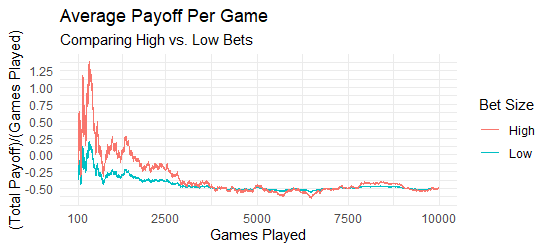
\includegraphics{Pictures/05-Expectations/highlowaveragepayoff.PNG}

We verify this using the formula for expected values (\ref{def:expectedvalue}):
\[.25 \cdot 28+.75 \cdot {-10}=-.5\]

A difference between the lower and the higher bet sizes is that with the higher bet is that there are bigger wins and bigger losses. Notice in the graph below how the increases and decreases in money earned are larger with the higher bet size. In this example the higher bet size has the same mean but a higher \textbf{variance}

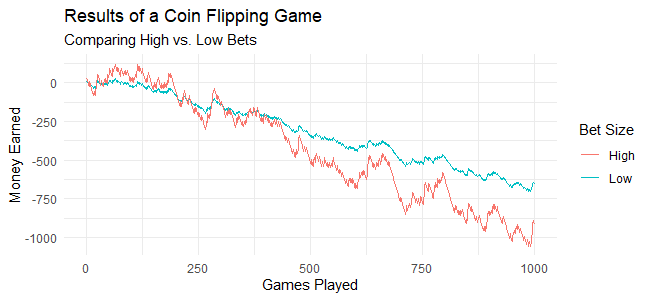
\includegraphics{Pictures/05-Expectations/highlowbets.PNG}

\hypertarget{defining-variance}{%
\subsection{Defining Variance}\label{defining-variance}}

\begin{center}\rule{0.5\linewidth}{0.5pt}\end{center}

\BeginKnitrBlock{definition}[Definition of Variance]
\protect\hypertarget{def:variance}{}{\label{def:variance} \iffalse (Definition of Variance) \fi{} }The variance of a random variable \(X\) is denoted by \(V(X)\). It is defined as:
\[V(X)=E((X-\mu )^2) = \sum (x - \mu)^2 \cdot p(x)\]
\EndKnitrBlock{definition}

\begin{center}\rule{0.5\linewidth}{0.5pt}\end{center}

Let \(X\) be the payoff of the smaller bet sizes and \(Y\) be the payoff for the larger bet sizes. We calculate the variance of the payoff for both games.

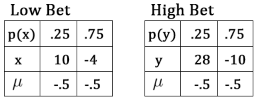
\includegraphics{Pictures/05-Expectations/highlow_variance_table.PNG}

\[V(X) = E((X-\mu)^2) = .25 \cdot (10 - ({-.5}))^2 + .75 \cdot ({-4} - (-.5))^2 = 36.75\]
\[V(Y) = E((Y-\mu)^2) = .25 \cdot (28 - ({-.5}))^2 + .75 \cdot ({-10} - (-.5))^2 = 270.75\]

The game with the larger bet sizes has a larger variance, agreeing with our experiments

\begin{center}\rule{0.5\linewidth}{0.5pt}\end{center}

\BeginKnitrBlock{exercise}
\protect\hypertarget{exr:unnamed-chunk-17}{}{\label{exr:unnamed-chunk-17} }Let \(X\) be \(1\) if a coin flips heads and \(0\) if it is tails. Show that the \(V(X) = .25\).
\EndKnitrBlock{exercise}

\begin{center}\rule{0.5\linewidth}{0.5pt}\end{center}

\hypertarget{variance-intuition}{%
\subsection{Variance Intuition}\label{variance-intuition}}

Consider that \(V(X)=\sum (x - \mu)^2 \cdot p(x)\). \((x - \mu)^2\) is the area of a square with sides of length \(x - \mu\). \(V(X)=\sum (x - \mu)^2 \cdot p(x)\) is then the probability weighted sum of the area of squares. Do you see why the larger bet sizes cause a larger variance?

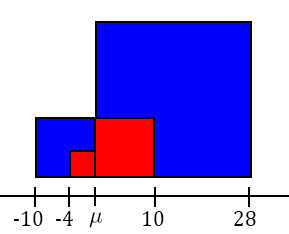
\includegraphics{Pictures/05-Expectations/squares.PNG}

\hypertarget{vaxb}{%
\subsection{V(aX+b)}\label{vaxb}}

Suppose we flip a coin once. We receive \(2\$\) if the coin is heads. Let \(X\) be \(1\) if heads and \(0\) otherwise, and \(Y\) be the number of doillars received. Note that \(Y=2X\). \(E(Y)=1\) and \(E(X)=.5\), remember that these numbers appear in our variance formula as \(\mu\). We calculate \(V(X)\) and \(V(Y)\):
\[V(X) = .5 \cdot (0-.5)^2 + .5 \cdot (1-.5)^2=.25\]
\[V(Y) = .5 \cdot (0-1)^2 + .5 \cdot (2-1)^2=1\]

There is a good reason that \(V(Y) = V(2X)= 2^2\cdot V(X)\)

\begin{align} 
V(Y) &= .5 \cdot (0-1)^2 + .5 \cdot (2-1)^2 \notag \\
&= .5 \cdot (2 \cdot 0- 2 \cdot .5)^2 + .5 \cdot (2 \cdot 1-2 \cdot .5)^2 \notag \\
&= 2^2 \cdot (.5 \cdot (0-.5)^2 + .5 \cdot (1-.5)^2) \notag \\
&= 2^2 \cdot V(X)
\end{align}

In general it is true that \(V(aX) = a^2 V(X)\). The manipulations performed in the coin flipping example could be applied anywhere.

What if we make a new random variable \(Z\) where we make \(2\$\) for heads and \(1\$\) dollars for tails? In this case \(Z = X+1\). We calculate \(V(Z)\), note that \(E(Z)=E(X+1)=E(X)+1=1.5\):
\[V(Z) = .5 \cdot (1-1.5)^2 + .5 \cdot (2-1.5)^2=.25\]
\(V(Z)=V(X)\) because the values are spread out the same distance. In general \(V(X+b) = V(X)\) because the translation does not change how far apart the values are. If you are feeling inspired try to write a proof of this.

Combining these observations we get the following theorem.

\begin{center}\rule{0.5\linewidth}{0.5pt}\end{center}

\BeginKnitrBlock{theorem}[V(aX+b)]
\protect\hypertarget{thm:unnamed-chunk-18}{}{\label{thm:unnamed-chunk-18} \iffalse (V(aX+b)) \fi{} }For a random variable \(X\) with constants \(a\) and \(b\):
\[V(aX+b) = a^2 V(X)\]
\EndKnitrBlock{theorem}

\begin{center}\rule{0.5\linewidth}{0.5pt}\end{center}

\begin{center}\rule{0.5\linewidth}{0.5pt}\end{center}

\BeginKnitrBlock{exercise}
\protect\hypertarget{exr:unnamed-chunk-19}{}{\label{exr:unnamed-chunk-19} }Show that \(V(-2X+1) = 4V(X)\).
\EndKnitrBlock{exercise}

\begin{center}\rule{0.5\linewidth}{0.5pt}\end{center}

\hypertarget{common-discrete-distributions}{%
\chapter{Common Discrete Distributions}\label{common-discrete-distributions}}

\hypertarget{bernoulli-distribution}{%
\section{Bernoulli Distribution}\label{bernoulli-distribution}}

The Bernoulli distribution is appropriate when there are two outcomes. Success happens with probability \(p\) and failure happens with probability \(1-p\).
\begin{equation*} 
    p(x) =
    \left\{
        \begin{array}{cc}
                p & \mathrm{for\ } x=1 \\
                1-p & \mathrm{for\ } x=0 \\
        \end{array} 
    \right.
\label{eq:bernoulli}
\end{equation*}

\begin{center}\rule{0.5\linewidth}{0.5pt}\end{center}

\BeginKnitrBlock{exercise}
\protect\hypertarget{exr:bernoulli}{}{\label{exr:bernoulli} }Let \(X\) be a Bernoulli random variable. Show that \(E(X)=p\) and that \(V(X)=p \cdot (1-p)\).
\EndKnitrBlock{exercise}

\begin{center}\rule{0.5\linewidth}{0.5pt}\end{center}

The number of heads from a single coin flip is an example of a Bernoulli random variable. The event that the coin lands on heads is success, tails is failure. If the coin is fair, \(p\) = .5.

\hypertarget{binomial-distribution}{%
\section{Binomial Distribution}\label{binomial-distribution}}

We have an unfair coin that is heads \(60\%\) of the time and tails \(40\%\) of the time. We flip the coin \(5\) times. We express the number of heads as the sum of Bernoulli random variables, \(X = H_1 + H_2 + H_3 + H_4 + H_5\) where
\begin{equation*} 
    H_i =
    \left\{
        \begin{array}{cc}
                1 \text{ if flip } i \text{ is heads} \\
                0 \text{ if flip } i \text{ is tails} \\
        \end{array} 
    \right.
\end{equation*}

We wish to calculate the probability that all \(5\) flips are heads. Because coin flips are independent we can use the rule \(P(A \cap B) = P(A) \cdot P(B)\)
\begin{align} 
P(X=5) &= P((H_1=1) \cap (H_2=1) \cap (H_3=1) \cap (H_4=1) \cap (H_5=1)) \notag \\
&=P(H_1=1) \cdot P(H_2=1) \cdot P(H_3=1) \cdot P(H_4=1) \cdot P(H_5=1)  \notag \\
&= .6^5 \notag
\end{align}

Less formally, the only way to achieve all heads is to flip the sequence \(HHHHH\). Each head happens with probability \(.6\) and the answer is \(.6^5\).

What about the probability of flipping exactly \(4\) heads? The sequences that can lead to this outcome are:
\begin{align} 
THHHH \notag \\
HTHHH  \notag \\
HHTHH \notag \\
HHHTH \notag \\
HHHHT \notag
\end{align}

These sequences all represent distinct outcomes for \(X\). Although some of the sequences are the same in some places, each represents a distinct outcome of \(X\), disjoint from all other outcomes. So we can use the addition formula for the probability of disjoint events.
\begin{align} 
&P(X=4) = \notag \\
&P((THHHH) \cup (HTHHH) \cup (HHTHH) \cup (HHHTH) \cup (HHHHT)) = \notag \\
&P(THHHH) + P(HTHHH) + P(HHTHH) + P(HHHTH) + P(HHHHT)=  \notag \\
&5 \cdot .6^4 \cdot .4 \notag
\end{align}

What about the probability of \(3\) heads? There are many sequences of flips that result in this, like \(HTHTH\). Each of these sequences will have probability \(.6^3 \cdot .4^2\) because there are three heads and two tails. To find out how many sequences there are we must answer the question ``How many ways are there to assign three of the five coins to be heads?'' The answer to this question is:
\[{5 \choose 3} = \frac{5!}{3!2!} = 10\]
There are \({5 \choose 3}\) ways to flip \(3\) heads and each way has probability \(.6^3 \cdot .4^2\), so the probability of three heads is \({5 \choose 3} \cdot .6^3 \cdot .4^2\).

This technique works for the other calculations we have done. There are \({5 \choose 5} = \frac{5!}{5!0!}=1\) ways to flip \(5\) heads and \({5 \choose 4} = \frac{5!}{4!1!}=5\) ways to flip \(4\) heads.

Let's generalize from our coin flipping. We had \(5\) independent Bernoulli trials where each Bernoulli trial had a probability of success as \(.6\). What if we had \(n\) Bernoulli trials each with a probability of success of \(p\). This is called the \textbf{binomial distribution} with parameters \(n\) and \(p\).

\begin{center}\rule{0.5\linewidth}{0.5pt}\end{center}

\BeginKnitrBlock{theorem}[Binomial Distribution]
\protect\hypertarget{thm:unnamed-chunk-20}{}{\label{thm:unnamed-chunk-20} \iffalse (Binomial Distribution) \fi{} }Let \(X\) have the binomial distribution with parameters \(n\) and \(p\). We have:
\[p(k) = P(X=k) = {n \choose k}p^k(1-p)^{n-k}\]
\EndKnitrBlock{theorem}

\begin{center}\rule{0.5\linewidth}{0.5pt}\end{center}

Be sure that this makes perfect sense.

\hypertarget{mean-and-variance-of-the-binomial-distribution}{%
\subsection{Mean and Variance of the Binomial Distribution}\label{mean-and-variance-of-the-binomial-distribution}}

In exercise \ref{exr:bernoulli} the motivated student showed that if \(X\) is Bernoulli with parameter \(p\) then \(E(X) = p\) and \(V(X) = p(1-p)\). These formulas for the binomial distribution are very similar.

\begin{center}\rule{0.5\linewidth}{0.5pt}\end{center}

\BeginKnitrBlock{theorem}[Binomial Distribution]
\protect\hypertarget{thm:unnamed-chunk-21}{}{\label{thm:unnamed-chunk-21} \iffalse (Binomial Distribution) \fi{} }Let \(X\) have the binomial distribution with parameters \(n\) and \(p\). We have:
\[E(X) = np\]
\[V(X) = np(1-p)\]
\EndKnitrBlock{theorem}

\begin{center}\rule{0.5\linewidth}{0.5pt}\end{center}

\hypertarget{intuition}{%
\subsubsection{Intuition}\label{intuition}}

Let \(X\) be the number of heads from a single coin flip. Let \(Y\) be the number of heads from \(10\) coin flips.
\[E(X)=p=.5\]
\[E(Y)=np=10 \cdot .5\]

We can express \(Y\) as the sum of single coin flips so \(Y = X_1 + ... + X_{10}\). I feel like I could have guessed that \(E(Y)=E(X_1 + ... + X_{10})\)

\backmatter
  \bibliography{book.bib,packages.bib}

\end{document}
